
\noindent \textbf{L5.1} Construa a gramática obtida a partir do autômato a pilha da figura 2.15 usando o lema 2.27, a segunda parte do teorema 2.20. Particione o conjunto de variáveis da sua gramática de forma a exibir quais delas geram a linguagem vazia e quais geram linguagens não vazias.\\[3pt]
\textbf{Resposta: } Referência em \cite{portland}. O autômato dado na figura 2.15 não atende às três condições solicitadas no lema 2.27, a saber:

\begin{enumerate}[label={\textbf{\arabic*.}}]
    \item Deve ter um  único estado de aceitação
    \item A pilha deve estar vazia ao aceitar
    \item Toda transição ou empilha, ou desempilha um símbolo
\end{enumerate}

Claramente o autômato não atende à condição 1. Podemos adicionar uma transição $\epsilon, \epsilon \rightarrow \epsilon$ de $q_1$ a $q_4$ para que $q_1$ deixe de ser um estado de aceitação, porém, o novo autômato não atenderia à condição 3. Logo, vamos adicionar um estado intermediário entre $q_1$ e $q_4$ e transições que empilham e desempilham o símbolo $\texttt{\#}$, respectivamente. Note que essa alteração faz com que o  autômato atenda às 3 condições solicitadas.

\begin{center}
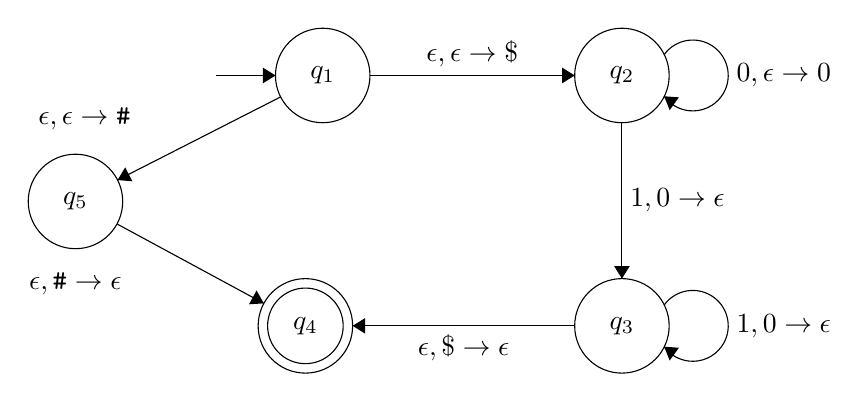
\begin{tikzpicture}[scale=0.2]
\tikzstyle{every node}+=[inner sep=0pt]
\draw [black] (34.3,-14.5) circle (3);
\draw (34.3,-14.5) node {$q_1$};
\draw [black] (18.6,-22.5) circle (3);
\draw (18.6,-22.5) node {$q_5$};
\draw [black] (33.2,-30.4) circle (3);
\draw (33.2,-30.4) node {$q_4$};
\draw [black] (33.2,-30.4) circle (2.4);
\draw [black] (53.3,-14.5) circle (3);
\draw (53.3,-14.5) node {$q_2$};
\draw [black] (53.3,-30.4) circle (3);
\draw (53.3,-30.4) node {$q_3$};
\draw [black] (27.5,-14.5) -- (31.3,-14.5);
\fill [black] (31.3,-14.5) -- (30.5,-14) -- (30.5,-15);
\draw [black] (31.63,-15.86) -- (21.27,-21.14);
\fill [black] (21.27,-21.14) -- (22.21,-21.22) -- (21.76,-20.33);
\draw (19.17,-17.97) node [above] {$\epsilon, \epsilon \rightarrow \texttt{\#}$};
\draw [black] (21.24,-23.93) -- (30.56,-28.97);
\fill [black] (30.56,-28.97) -- (30.1,-28.15) -- (29.62,-29.03);
\draw (18.59,-26.97) node [below] {$\epsilon, \texttt{\#} \rightarrow \epsilon$};
\draw [black] (50.3,-30.4) -- (36.2,-30.4);
\fill [black] (36.2,-30.4) -- (37,-30.9) -- (37,-29.9);
\draw (43.25,-30.9) node [below] {$\epsilon, \$ \rightarrow \epsilon$};
\draw [black] (55.98,-29.077) arc (144:-144:2.25);
\draw (60.55,-30.4) node [right] {$1, 0 \rightarrow \epsilon$};
\fill [black] (55.98,-31.72) -- (56.33,-32.6) -- (56.92,-31.79);
\draw [black] (55.98,-13.177) arc (144:-144:2.25);
\draw (60.55,-14.5) node [right] {$0, \epsilon \rightarrow 0$};
\fill [black] (55.98,-15.82) -- (56.33,-16.7) -- (56.92,-15.89);
\draw [black] (37.3,-14.5) -- (50.3,-14.5);
\fill [black] (50.3,-14.5) -- (49.5,-14) -- (49.5,-15);
\draw (43.8,-14) node [above] {$\epsilon, \epsilon \rightarrow \$$};
\draw [black] (53.3,-17.5) -- (53.3,-27.4);
\fill [black] (53.3,-27.4) -- (53.8,-26.6) -- (52.8,-26.6);
\draw (53.8,-22.45) node [right] {$1, 0 \rightarrow \epsilon$};
\end{tikzpicture}
\end{center}

Seja $Q = \{q_1, q_2, q_3,q_4, q_5\}$ o conjunto de estados do autômato acima modificado. Vamos denominar por $G$ a gramática que vamos construir a partir do autômato de acordo com o procedimento dado no lema 2.27. A regra inicial é:

$S \rightarrow A_{14}$

\begin{enumerate}[label={\textbf{\arabic*.}}]
    \item Para cada $p \in Q$, insira a regra $A_{pp} \rightarrow \epsilon$ em $G$\\[2pt]
    $A_{11} \rightarrow \epsilon$\\
    $A_{22} \rightarrow \epsilon$\\
    $A_{33} \rightarrow \epsilon$\\
    $A_{44} \rightarrow \epsilon$\\
    $A_{55} \rightarrow \epsilon$
    
    \item Para cada $p, q, r \in Q$, insira a regra $A_{pq} \rightarrow A_{pr}A_{rq}$ em $G$\\[2pt]
    $A_{11} \rightarrow A_{11}A_{11}\ |\ A_{12}A_{21}\ |\ A_{13}A_{31}\ |\ A_{14}A_{41}\ |\ A_{15}A_{51}$\\
    $A_{12} \rightarrow A_{11}A_{12}\ |\ A_{12}A_{22}\ |\ A_{13}A_{32}\ |\ A_{14}A_{42}\ |\ A_{15}A_{52}$\\
    $A_{13} \rightarrow A_{11}A_{13}\ |\ A_{12}A_{23}\ |\ A_{13}A_{33}\ |\ A_{14}A_{43}\ |\ A_{15}A_{53}$\\
    $A_{14} \rightarrow A_{11}A_{14}\ |\ A_{12}A_{24}\ |\ A_{13}A_{34}\ |\ A_{14}A_{44}\ |\ A_{15}A_{54}$\\
    $A_{15} \rightarrow A_{11}A_{15}\ |\ A_{12}A_{25}\ |\ A_{13}A_{35}\ |\ A_{14}A_{45}\ |\ A_{15}A_{55}$\\[4pt]
    $A_{21} \rightarrow A_{21}A_{11}\ |\ A_{22}A_{21}\ |\ A_{23}A_{31}\ |\ A_{24}A_{41}\ |\ A_{25}A_{51}$\\
    $A_{22} \rightarrow A_{21}A_{12}\ |\ A_{22}A_{22}\ |\ A_{23}A_{32}\ |\ A_{24}A_{42}\ |\ A_{25}A_{52}$\\
    $A_{23} \rightarrow A_{21}A_{13}\ |\ A_{22}A_{23}\ |\ A_{23}A_{33}\ |\ A_{24}A_{43}\ |\ A_{25}A_{53}$\\
    $A_{24} \rightarrow A_{21}A_{14}\ |\ A_{22}A_{24}\ |\ A_{23}A_{34}\ |\ A_{24}A_{44}\ |\ A_{25}A_{54}$\\
    $A_{25} \rightarrow A_{21}A_{15}\ |\ A_{22}A_{25}\ |\ A_{23}A_{35}\ |\ A_{24}A_{45}\ |\ A_{25}A_{55}$\\[4pt]
    $A_{31} \rightarrow A_{31}A_{11}\ |\ A_{32}A_{21}\ |\ A_{33}A_{31}\ |\ A_{34}A_{41}\ |\ A_{35}A_{51}$\\
    $A_{32} \rightarrow A_{31}A_{12}\ |\ A_{32}A_{22}\ |\ A_{33}A_{32}\ |\ A_{34}A_{42}\ |\ A_{35}A_{52}$\\
    $A_{33} \rightarrow A_{31}A_{13}\ |\ A_{32}A_{23}\ |\ A_{33}A_{33}\ |\ A_{34}A_{43}\ |\ A_{35}A_{53}$\\
    $A_{34} \rightarrow A_{31}A_{14}\ |\ A_{32}A_{24}\ |\ A_{33}A_{34}\ |\ A_{34}A_{44}\ |\ A_{35}A_{54}$\\
    $A_{35} \rightarrow A_{31}A_{15}\ |\ A_{32}A_{25}\ |\ A_{33}A_{35}\ |\ A_{34}A_{45}\ |\ A_{35}A_{55}$\\[4pt]
    $A_{41} \rightarrow A_{41}A_{11}\ |\ A_{42}A_{21}\ |\ A_{43}A_{31}\ |\ A_{44}A_{41}\ |\ A_{45}A_{51}$\\
    $A_{42} \rightarrow A_{41}A_{12}\ |\ A_{42}A_{22}\ |\ A_{43}A_{32}\ |\ A_{44}A_{42}\ |\ A_{45}A_{52}$\\
    $A_{43} \rightarrow A_{41}A_{13}\ |\ A_{42}A_{23}\ |\ A_{43}A_{33}\ |\ A_{44}A_{43}\ |\ A_{45}A_{53}$\\
    $A_{44} \rightarrow A_{41}A_{14}\ |\ A_{42}A_{24}\ |\ A_{43}A_{34}\ |\ A_{44}A_{44}\ |\ A_{45}A_{54}$\\
    $A_{45} \rightarrow A_{41}A_{15}\ |\ A_{42}A_{25}\ |\ A_{43}A_{35}\ |\ A_{44}A_{45}\ |\ A_{45}A_{55}$\\[4pt]
    $A_{51} \rightarrow A_{51}A_{11}\ |\ A_{52}A_{21}\ |\ A_{53}A_{31}\ |\ A_{54}A_{41}\ |\ A_{55}A_{51}$\\
    $A_{52} \rightarrow A_{51}A_{12}\ |\ A_{52}A_{22}\ |\ A_{53}A_{32}\ |\ A_{54}A_{42}\ |\ A_{55}A_{52}$\\
    $A_{53} \rightarrow A_{51}A_{13}\ |\ A_{52}A_{23}\ |\ A_{53}A_{33}\ |\ A_{54}A_{43}\ |\ A_{55}A_{53}$\\
    $A_{54} \rightarrow A_{51}A_{14}\ |\ A_{52}A_{24}\ |\ A_{53}A_{34}\ |\ A_{54}A_{44}\ |\ A_{55}A_{54}$\\
    $A_{55} \rightarrow A_{51}A_{15}\ |\ A_{52}A_{25}\ |\ A_{53}A_{35}\ |\ A_{54}A_{45}\ |\ A_{55}A_{55}$
    
    \item Por fim, para cada $p, q, r, s \in Q$, $t \in \Gamma$ e $a, b \in \Sigma_\epsilon$, insira a regra $A_{pq} \rightarrow aA_{rs}b$ em $G$, se $\delta(p, a, \epsilon)$ contém $(r, t)$ e $\delta(s, b, t)$ contém $(q, \epsilon)$\\[2pt]
    $A_{14} \rightarrow \epsilon A_{23} \epsilon\ |\ \epsilon A_{55} \epsilon$\\
    $A_{23} \rightarrow 0A_{22}1\ |\ 0A_{23}1$
\end{enumerate}

Com isso, concluímos a construção da gramática $G$.\\[6pt]

